SAM is a 2D guided model that requires a geometric prompt (or user prompt) to segment an image. The output is a set of segmentation masks at different levels and a confidence score for each. A segmentation mask is a 2D array with the same size as the image input. SAM consists of an encoder and a decoder. The encoder takes the image and geometric prompt to produce an image embedding, image position embedding, and geometric prompt embedding. The decoder takes in these various embeddings to produce segmentation masks and confidence scores.

\subsection{Geometric Prompts}
SAM supports three kinds of geometric prompts: points, bounding boxes, and dense masks. Points and bounding boxes are defined as sparse prompts, while dense masks are categorized as dense prompts.

\begin{itemize}
    \item A \textbf{point prompt} is a single pixel $(x, y)$. A positive point instructs the model to include the point in the produced segmentation mask, whereas a negative point instructs the model to exclude the pixel. The model accepts multiple points to guide the segmentation.
    
    \item A \textbf{bounding box} is defined by a top-left corner $(x_1, y_1)$ and a bottom-right corner $(x_2, y_2)$. Bounding boxes are always treated as positive prompts, instructing the model to produce the segment within the boxed area. Multiple bounding boxes may be provided.
    
    \item \textbf{Dense masks} are represented as a low-resolution 2D grid of size $256 \times 256 \times 1$. Each entry contains a floating-point value in the range $[0, 1]$, representing the probability that a pixel belongs to the segment mask.
\end{itemize}


\subsection{Prompt Embeddings}
\begin{figure}[!h]
    \centering
    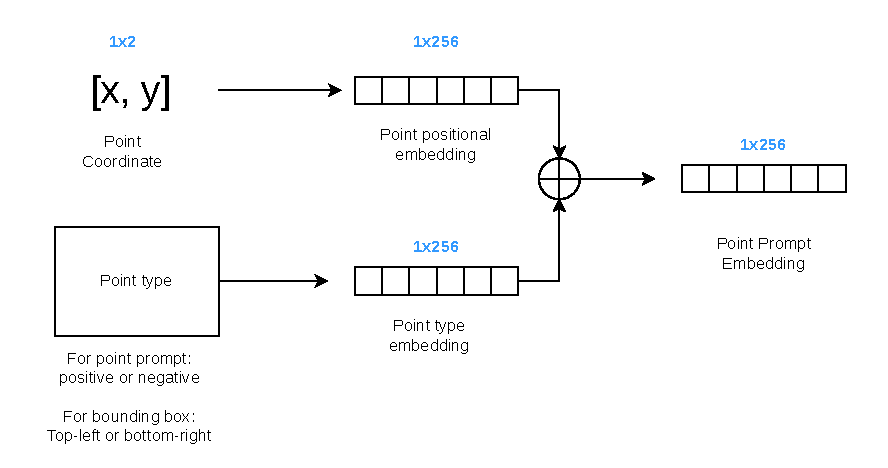
\includegraphics[width=1\textwidth]{graphics/background/point_embedding.pdf}
    \caption{Point Prompt Embedding}
    \label{fig:point_embedding}
\end{figure}


The PromptEncoder module in SAM maps geometric prompts to a latent space $\mathbb{R}^{256}$. Figure \ref{fig:point_embedding} illustrates the point prompt encoding process. It generates a positional encoding from spatial coordinates and a type embedding, each 
utilizing 256 trainable parameters. These vectors are combined via element-wise addition to produce the final 256-dimensional prompt embedding. All positive clicks use the same learned ``positive" vector, while negative clicks 
use a ``negative" vector. These 512 parameters are optimized during the training phase.

Similarly, bounding boxes are represented as a pair of point embeddings. To distinguish 
them from standard point prompts, SAM employs specific learned embeddings for the 
``top-left" and ``bottom-right" corners, resulting in two 256-dimensional vectors.

For the dense mask, the PromptEncoder downscales $256 \times 256 \times 1$ masks into dense embeddings 
of shape $256 \times 64 \times 64$, which are subsequently added element-wise to the 
image embeddings.

\subsection{Image Embeddings}
Figure \ref{fig:image_embedding} illustrates how SAM embed the image. The \texttt{ImageEncoderViT} accepts a raw input image, resizing it to a fixed resolution of $1024 \times 1024$. This input is processed into a $64 \times 64$ feature grid, creating a dense image embedding with a feature dimension of $256$. Within the \texttt{ImageEncoderViT}, various trainable parameters facilitate this transformation.

Simultaneously, the \texttt{PromptEncoder} generates positional embeddings for all $64 \times 64$ coordinates, resulting in an image positional embedding of shape $64 \times 64 \times 256$. The image content embedding tensor and its corresponding positional embedding are combined via element-wise addition to produce the final embedding. This final representation encapsulates both the semantic image 
information and the spatial positional information for all pixels. 

\begin{figure}[!h]
    \centering
    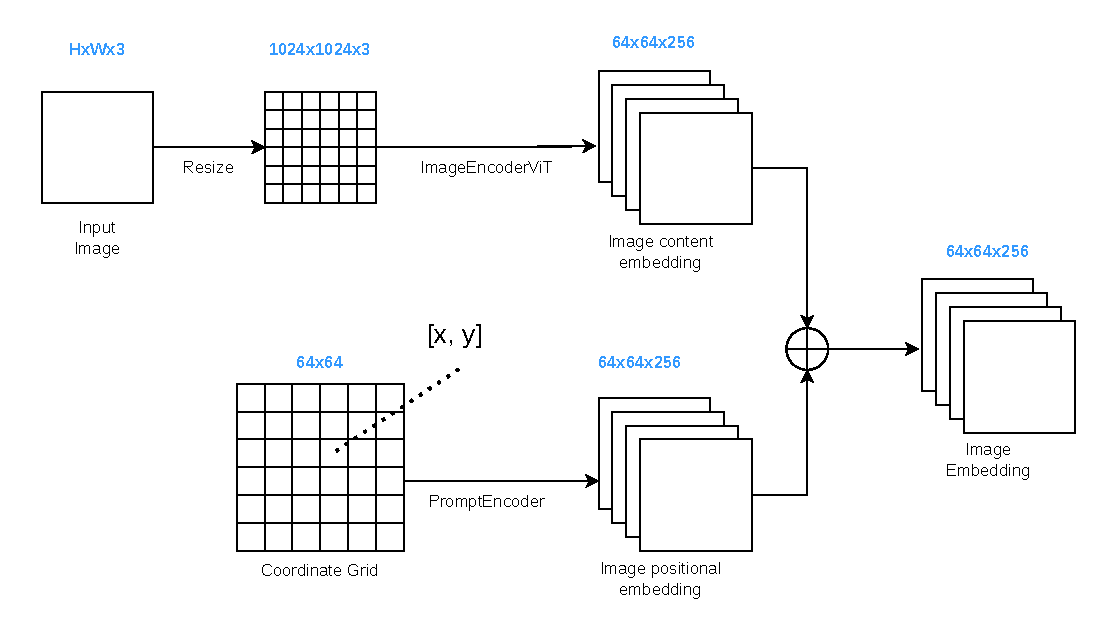
\includegraphics[width=1\textwidth]{graphics/background/image_embedding.pdf}
    \caption{Image Embedding}
    \label{fig:image_embedding}
\end{figure}

\subsection{Decoder}
The decoder inputs consist of the image positional embeddings, the image embedding, the dense mask embedding, and the sparse prompts. The image embedding and dense mask embedding are combined via element-wise addition to produce a $256 \times 64 \times 64$ tensor as input for the two-way transformer. The decoder also initializes a $1 \times 256$ IoU token and a $4 \times 256$ mask token from PyTorch's ``Embedding'' module. The figure \ref{fig:decoder} illustrates the decoding process.

The IoU token is not connected to any user input. During the transformer's processing, it is treated as an additional input along with the four mask tokens. It participates in the same two-way cross-attention layers, allowing it to attend to both the sparse prompt embeddings and the dense image features. This process enables the token to gather global context regarding how well the predicted mask aligns with the image data.

The four mask tokens serve as queries for the transformer. The attended mask tokens finally produce segmentation mask prediction heads for the four levels of masks. Three multi-mask tokens are designed for the ``subpart,'' ``part,'' and ``whole'' hierarchical levels, while the other token is optimized for unambiguous prompts, such as when a dense mask is already provided.

\begin{figure}[!h]
    \centering
    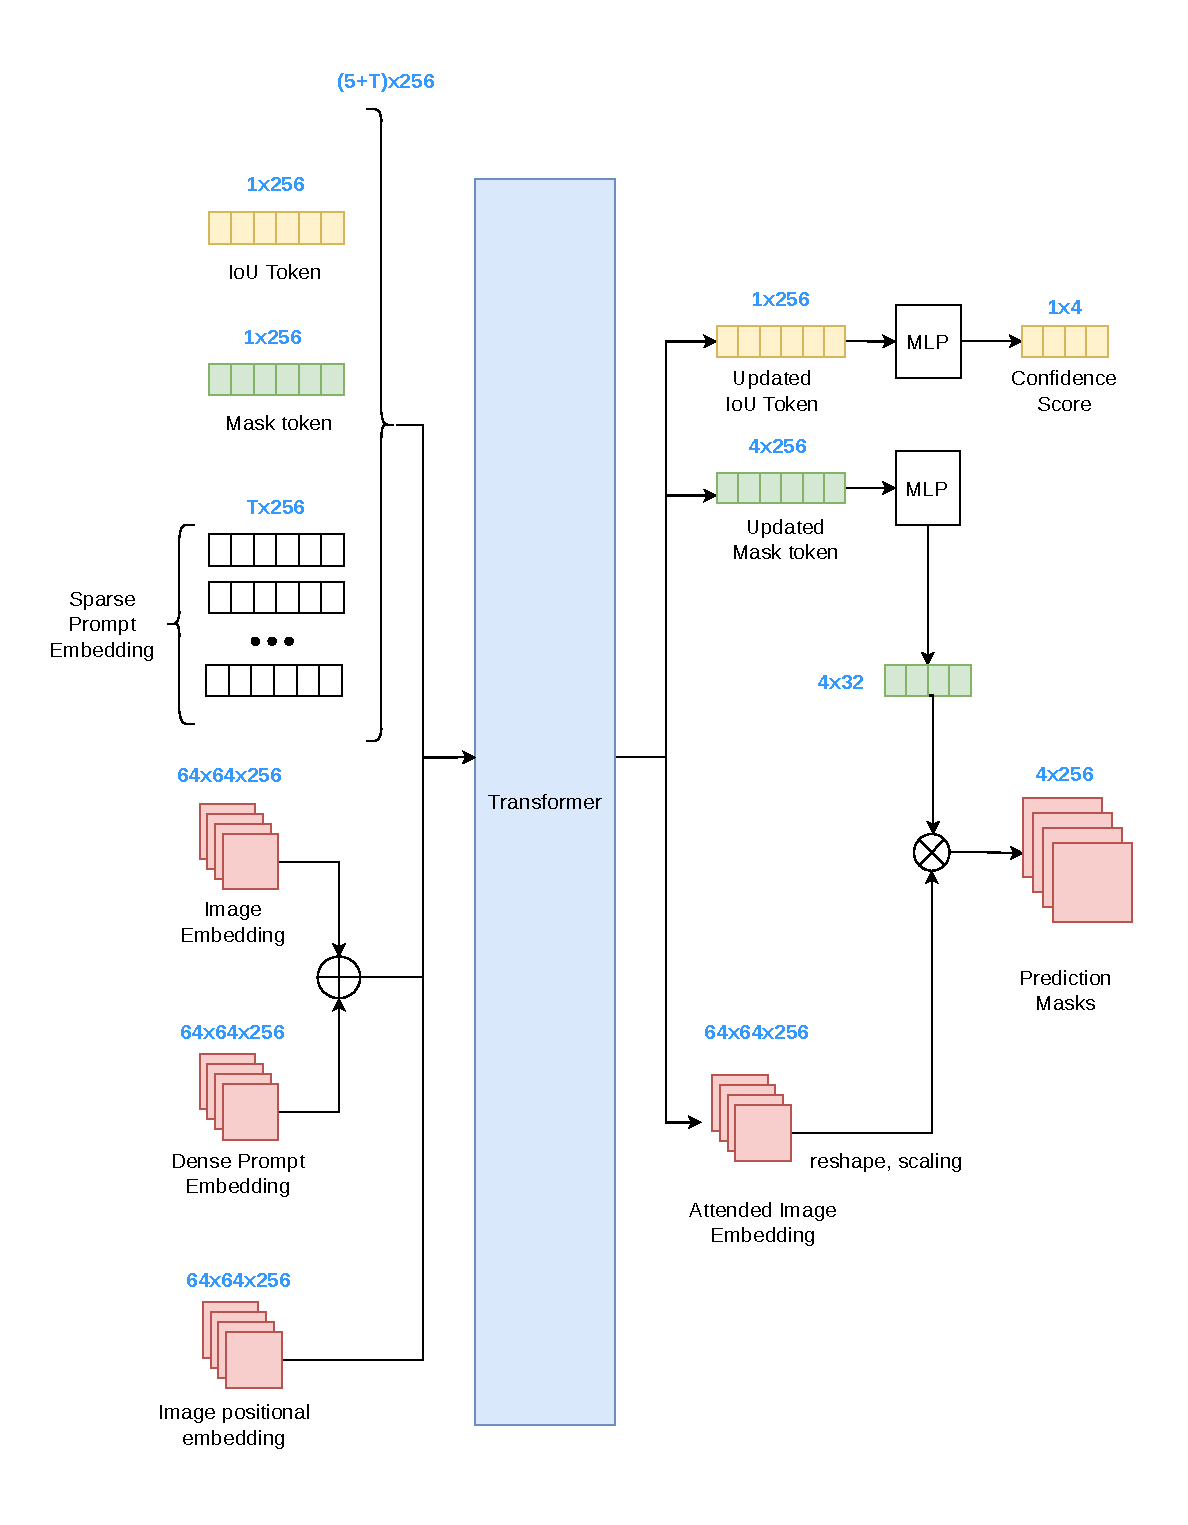
\includegraphics[width=1\textwidth]{graphics/background/decoder.pdf}
    \caption{Mask Decoder Process}
    \label{fig:decoder}
\end{figure}




\section{Parameter Efficient Fine-Tuning Techniques}
\subsection{LoRa}
To maintain the foundational knowledge of the pre-trained Segment Anything Model (SAM) while specializing it for meteorological features, we utilize Low-Rank Adaptation (LoRA)[cite: 341]. This approach is particularly effective for adapting SAM to the ClimateNet domain, as it allows for domain-specific refinement without the prohibitive computational cost of full parameter fine-tuning[cite: 301, 341].

\subsubsection{Conceptual Framework}
LoRA operates on the principle that the updates to the weights during adaptation have a low ``intrinsic rank". Instead of updating the massive original weight matrix $W$, we represent the update $\Delta W$ as the product of two much smaller, trainable matrices, $A$ and $B$. For a given input $x$, the modified forward pass is calculated as:

\begin{equation}
    y = Wx + \Delta Wx = Wx + BAx
\end{equation}

During the training phase, the original weight matrix $W$ remains frozen, and only the low-rank matrices $A$ and $B$ are updated. This significantly reduces the number of trainable parameters while allowing the model to capture the complex, non-image atmospheric patterns of Tropical Cyclones and Atmospheric Rivers.

\subsubsection{Implementation Details}
Our implementation focuses on injecting these adapters into the Transformer blocks of the SAM image encoder. Specifically, we target the Query ($q$) and Value ($v$) projection layers within the multi-head self-attention mechanism, as these layers are critical for internalizing the spatial relationships of weather phenomena.

\begin{itemize}
    \item \textbf{Rank Selection}: We utilize a small rank $r$ to ensure the adaptation remains efficient and prevents over-fitting to the sparse labels in the ClimateNet dataset.
    \item \textbf{Layer Injection}: Adapters are placed in parallel with the original linear layers, specifically targeting the $q$ and $v$ slices of the $qkv$ projection.
    \item \textbf{Initialization}: Matrix $A$ is initialized using a Kaiming uniform distribution to provide a stable starting gradient, while Matrix $B$ is initialized to zero. This ensures that at the beginning of training, the "shortcut" has zero impact, and the model starts with the exact behavior of the vanilla SAM.
\end{itemize}

\subsubsection{Strategic Advantages}
By employing LoRA, we isolate the adaptation process of the encoder[cite: 343]. This methodology ensures that the model focuses exclusively on learning to extract high-quality, diagnostic features from the 16 multi-parameter atmospheric grids[cite: 344]. This is vital for recognizing the "ribbon-like" corridors of ARs and the "circular" structures of TCs, which differ significantly from the high-frequency edges found in traditional RGB images[cite: 345].

\subsection{Learnable Token}
In CAT-SAM-T and HQ-SAM, a small learnable token of dimension 1×256 is introduced \cite{xiao2024cat, ke2023segment}. This token is combined via element-wise addition with the original IoU token embedding to initialize a refined IoU token. Following processing through the transformer blocks, the updated token incorporates global image context, critical geometric and categorical information from the prompt tokens, and latent mask information from other output tokens. The refined token is then passed through an MLP and subsequently undergoes a spatially point-wise product with the fused image features to facilitate high-quality mask generation.
